\documentclass[12pt]{article}
\usepackage[paper=a4paper,left=20mm,right=20mm,top=30mm,bottom =30mm]{geometry}
\usepackage[utf8]{inputenc}
\usepackage[T1]{fontenc}
\usepackage{stmaryrd}
\usepackage{setspace}
\usepackage{mathrsfs}
\usepackage[ngerman]{babel}
\usepackage{amssymb}
\usepackage{amsmath}
\usepackage{fancyhdr}
\usepackage[dvips,unicode,colorlinks,linkcolor=black]{hyperref} 
\usepackage{graphicx}
\usepackage{float}

\pagestyle{fancy}
\lfoot{}
\rfoot{Paul Kremser, Tobias Grussenmeyer}
\cfoot{\thepage}
\fancyhead[L]{FPI Versuch: Ultraschall}
\renewcommand{\headrulewidth}{0.6pt}
\renewcommand{\footrulewidth}{0.6pt}
\setlength{\headheight}{16pt}
\setlength{\parindent}{0pt}
% Für die Wahl der Schriftart
\newcommand{\changefont}[3]{
\fontfamily{#1} \fontseries{#2} \fontshape{#3} \selectfont}

\begin{document}
% keine Hurenkinder und Schusterjungen
\clubpenalty = 10000
\widowpenalty = 10000 
\displaywidowpenalty = 10000

\onehalfspacing
% Schriftart
\changefont{ptm}{m}{n} 

\begin{titlepage}
\author{Paul Kremser, Tobias Grussenmeyer}
\title{Versuch: Ultraschall}
\date{Versuchsdurchführung: 6. und 7. Oktober 2009} 
\maketitle
\thispagestyle{empty}
\end{titlepage}


\tableofcontents
\thispagestyle{empty}
\newpage
\pagenumbering{arabic}
\section{Überblick}

\section{Aufgabestellung}
\textbf{Amplitudengitter}
\begin{itemize}
 \item Bestimmung der Gitterkonstante eines Sinusgitters aus dem Abstand des 1. Beugungsordnung
 \item Bestimmung der Gitterkonstanten von 5 Amplitudengittern
 \item Berechnung der Aperturfunktion für Gitter Nr. 1 (größte Gitterkonstante, höchste Dichte an Beugungsmaxima) aus den ermittelten Intensitäten
 der Beugungsordnungen und Zeichnen einer Periode der Aperturfunktion
 \item Bestimmung des Verhältnisses der Spaltbreite zum Spaltabstand aus der Aperturfunktion
 \item Bestimmung des Auflösevermögens der Gitter bei ihrer vollen Ausleuchtung
\end{itemize}

\textbf{Phasengitter}
\begin{itemize}
 \item Messung der Intensitätsverteilung der Beugungsfigur eines Ultraschallwellengitters (Phasengitter) in Abhängigkeit von der Spannung am
 Ultraschallschwingquarz
 \item Vergleich der Messergebnisse mit der Raman-Nath-Theorie
 \item Bestimmung der Schallwellenlänge in Isooktan durch Ausmessen der Beugungsordnungen un Vergleich mit dem rechnerischen Wert
\end{itemize}



\section{Theoretische Grundlagen}

\subsection{Beugung}
Unter Beugung versteht man eine Richtungsänderung elektromagnetischer Wellen an einem Hinderniss welche nicht von Reflexion oder Brechung herrührt. Dabei unterscheidet man zwischen zwei unterschiedlichen Versuchsanordnungen:
\begin{itemize}
 \item Fresnel’sche Anordnung: Bei dieser Anordnung ist der Abstand Lichtquelle-Apertur oder Schirm - Apertur klein, d.h. die Form der Wellenfront des einfallenden Lichts ist nicht vernachlässigbar.
 \item Frauenhofer Anordnung: Im Gegensatz zur Fresnelschen Anordnung sind hier die Abstände groß, d.h. die Wellenfront des einfallenden Lichts kann als eben angenommen werden. Zusätzlich wird gefordert, daß die Beugungsöffnung groß gegen die Wellenlänge des einfallenden Lichtes ist.
\end{itemize}
Hier wird Beugung an Amplituden und Phasengittern an einer Frauenhofer Anordnung betrachtet.

\subsection{Amplitudengitter}
Jedes Gitter wird durch seine Gitterkonstante $K$ charakterisiert. Die Gitterkonstante gibt den Abstand zweier benachbarter Spaltmitten an.
Bei bekannter Wellenlänge $\lambda$ lässt sich die Gitterkonstante aus dem Winkel des $m$-ten Intensitätsmaximum gegenüber dem 0-ten Maximum berechnen:
\begin{align}
\label{gitterkonstante} K = \frac{m \ \lambda}{\sin{\theta}}
\end{align}

\subsection{Aperturfunktion}
Jedem Objekt, an dem Beugung stattfindet, lässt sich eine Aperturfunktion $g$ zuordnen. Die Aperturfunktion beschreibt die Eigenschaften des Objekts indem
sie jedem Punkt in der Blendenebene einen Wert zuorndet. Mit Hilfe des Kirchhoffschen Integraltheorems und der daraus erhaltenen Integralformel für die
Amplitude einer Kugelwelle auf dem Rand ihres Ausbreitungsgebietes kann man zeigen, dass die Fouriertransformierte der Aperturfunktion $g$ des
Beugungsobjekts gerade die Intensitätsverteilung $I$ des Beugungsbildes ist.
\begin{align}
 I = \lvert \Psi(x,y) \rvert^2 = \left\lvert \int_{Blende}{g \ e^{-ikr} \ dA} \right\rvert
\end{align}

Umgekehrt lässt sich durch Fouriertransformation aber auch die Aperturfunktion aus der Intensitätsverteilung gewinnen.
Die Fouriertransformierte einer Funktion ist wie folgt definiert:
\begin{align}
 F(g) = \int\limits_{-\infty}^{\infty}g(x)~e^{-ikx}~dx
\end{align}

Ist die genaue Intensitätsverteilung nicht vollständig bekannt so kann man die Aperturfunktion ersatzweise in einer Fourierreihe nähern.
Hierzu werden die Wurzeln der Intensitätsmaxima als Koeffizienten genommen:
\begin{align}
 g(x) = \sum_{j=0}^{\infty}{\pm \sqrt{I_j} \ \cos \left( \frac{x}{K} \ 2 \ \pi \ j \right) }
\end{align}

Bei einem Sinusgitter (hier treten nur Maxima 0-ter und 1-ter Ordnung auf) ergibt sich z.B.:
\begin{align*}
 g(x) = \sqrt{I_0} \ + \ \sqrt{I_1} \ \cos\left( \frac{x}{K} \ 2 \ \pi \right)
\end{align*}

Aus dem erhaltenen Graph die Aperturfunktion kann man dann die Spaltbreite und den Spaltabstand ablessen.

\subsection{Auflösungsvermögen}
Die Definition des Auflösungsvermögen $a$ ist:
\begin{align}
 a = \frac{\lambda}{\Delta\lambda}
\end{align}

mit der Wellenlänge $\lambda$ und dem Wellenlängenabstand $\Delta\lambda$ bei dem eine von $\lambda$ verschiedene Wellenlänge bei Beugung gerade noch
unterscheiden lässt. Zudem gilt:
\begin{align}
\label{auflösevermögen} a = N \ m
\end{align}
mit der Anzahl der augeleuchteten Gitterlinien $N$ und der größten beobachteten Beugungsordnung $m$.

\subsection{Phasengitter}
%VORHER: Die Beugung am Phasengitter ist in unserem Fall vernachlässigbar. Stattdessen wird der Strahl am Phasengitter unterschiedlich stark gebrochen.
Hier ist - im Gegensatz zum Amplitudengitter - die Transmission konstant, moduliert wird die Phase.
Eine Ultraschallwelle erzeugt in Isooktan Bereiche unterschiedlicher Dichte und somit unterschiedlicher Brechungsindizes.
Somit treten ehmals gleichphasige Wellen phasenverschoben aus dem Gitter aus und können miteinander interferieren. Für den brechungsindex $n$ in der 
Flüssigkeit gilt:
\begin{align}
 n(x) = n_0 + \Delta n \ sin\left(\frac{2\ \pi}{\Lambda}\ x\right)
\end{align}
mit $\Lambda$ der Schallwellenlänge, welche das Analogon dur Gitterkonstante beim Amplitudengitter ist.
Da $\Delta n$ proportional zur Schallintensität $S$ ist können wir den Brechungsindex mit der Amplitude der Schallwelle ändern.

\subsection{Raman-Nath-Theorie}
Für die Winkel der Intensitätsmaxima des Beugungsbildes gilt in $m$-ter Ordnung:
\begin{align}
 \sin~\theta = \pm~\frac{\lambda}{\Lambda}~m
\end{align}

Die Intensitäten der Maxima $m$-ter Ordnung verhalten sich zu denen $m'$-ter Ordnung wie die Besselfunktion der $m$-ten zu denen der $m'$-ten Ordnung.
\begin{align}
 \frac{I_m}{I_{m'}} = \frac{J^2_m(\Delta n~D \times 2~\pi~/~\lambda)}{J^2_{m'}(\Delta n \times 2~\pi~/~\lambda)}
\end{align}

\section{Versuchsaufbau}

\section{Durchführung}

\section{Auswertung}
\subsection{Gitterkonstante des Sinusgitters}
Bei der Beugung am Sinusgitter masen wir als Abstand zwischen den Beugungsordnungen $a=(4,7 \pm 0,1)cm$ und zwischen Gitter und Schirm masen wir $b=(5,7\pm0,2)cm$. Der Sinus ergibt sich aus a und der Hypothenuse des durch durchtrittspunkt auf dem Gitter, nullter und erster Ordnung auf dem Schirm gebildeten Dreiecks. Diese Hypothenuse ergibt sich zu $c=\sqrt{a^2+^2}$. Also folgt für den Winkel:
\begin{align}
\notag
 sin(\vartheta)=\frac{a}{c}=\frac{a}{\sqrt{a^2+b^2}}
\end{align}

nach Gleichung \ref{gitterkonstante} folgt also für Gitterkonstante K
\begin{align}
\notag
 K=\frac{\lambda}{sin(\vartheta)}=\frac{\lambda}{a}\sqrt{a^2+b^2}= \lambda\sqrt{\frac{b^2}{a^2}+1}
\end{align}

und für den Fehler $s_K$:
\begin{align}
\notag
 s_K=\sqrt{\frac{\partial K}{\partial a}s_a^2+\frac{\partial K}{\partial b}s_b^2}=\frac{b\lambda}{a^2}\sqrt{\frac{a^2s_b^2+b^2s_a^2}{a^2+b^2}}
\end{align}

Hiermit erhielten wir als Ergebnis die Gitterkonstante des Sinusgitters:
\begin{align}
\notag
 K=(9,95\pm0,24)\times10^{-7}m
\end{align}
\subsection{Gitterkonstanten der fünf Amplitudengitter}
Um die Gitterkonstante der 5 Amplitudengitter zu bestimmen musste zunächst die Zeitachse des Osziloskops in den Sinus des Ablenkwinkels umgerechnet werden. Hierfür wurde eine Eichmessung mit einem Referenzgitter R, dessen Gitterkonstante bekannt war durchgeführt. Die Angabe lautete 80 Linien pro cm, was einer Gitterkonstanten von $K_R=0,0125cm$ entspricht. Also lies sich mit Gleichung \ref{gitterkonstante} die Werte von $sin(\vartheta)$ zu den verschiedenen Ordnungen m berechnen. Diese trugen wir dann gegen die von uns gemessenen Zeitwerte auf und ermittelten, aus dem so entstehenden linearen Zusammenhang $sin(\vartheta)$, durch Geradenanpassung die Werte für a und b.

\begin{figure}[H]  
\centering
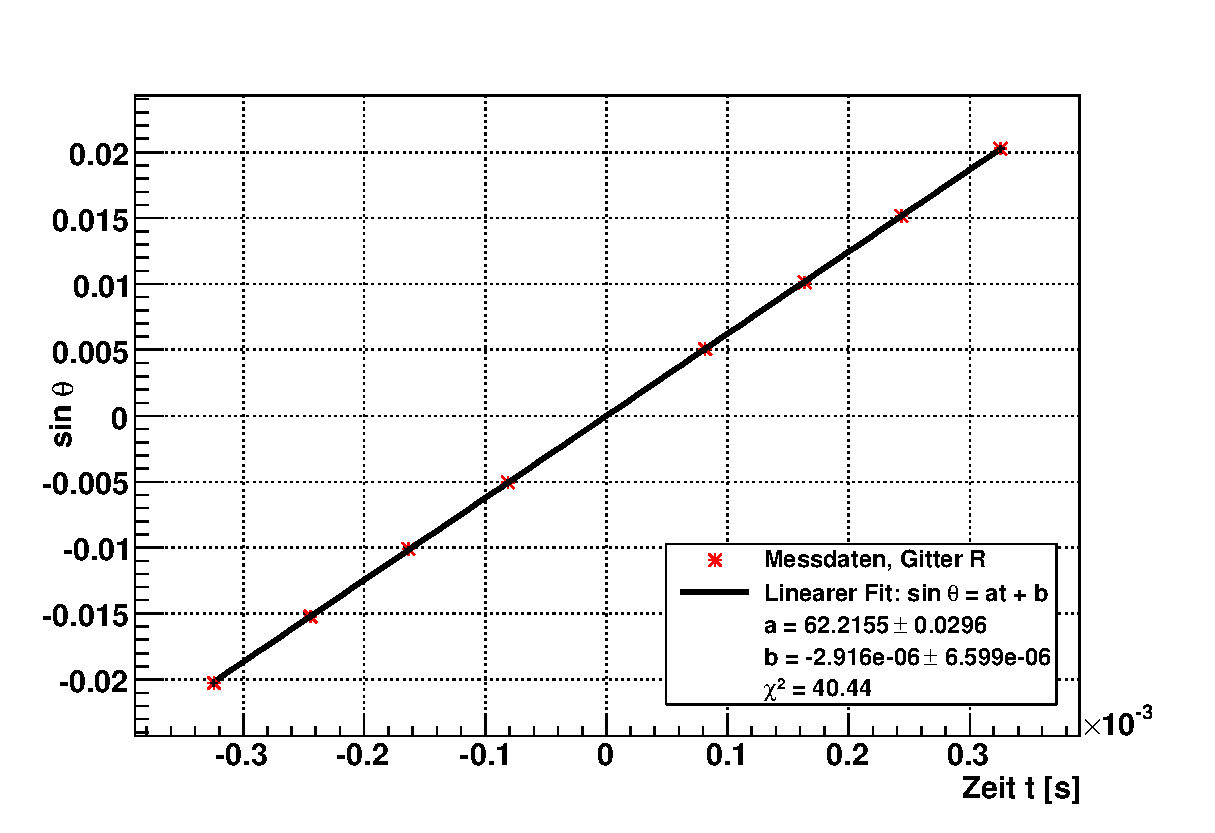
\includegraphics[width=0.7\linewidth]{pictures/r.eps}
\caption{Eichung der Zeitachse durch Referenzgitter}
\end{figure}

Aus diesem Fit erhält man also direkt die Umrechnung $sin(\vartheta)=at+b$ mit $a=(62,22\pm 0,03)s{-1}$ und $b=(2,92\pm 6,7)\times 10^{-6}$. Wir können also nun Anhand der Zeitskala auf den Sinus des Beugungswinkels der Gitter mit unbekanntem K rückschliessen. Der Fehler hierfür ergibt sich zu:
\begin{align}
 s_{sin(\vartheta)} = \sqrt{\frac{\partial sin(\vartheta)}{\partial t}^2s_t^2 + \frac{\partial sin(\vartheta)}{\partial a}^2s_a^2 + \frac{\partial sin(\vartheta)}{\partial b}^2s_b^2} = \sqrt{a^2s_t^2+t^2s_a^2+s_b^2}
\end{align}

Weiter lassen sich also nun auch über Gleichung \ref{gitterkonstante} die Gitterkonstanten $K_i$ für die fünf Amplitudengitter bestimmen. Dabei wird der lineare Zusammenhang 
\begin{align}
 sin(\vartheta) = \frac{\lambda}{K_i}m = a_im
\end{align}
ausgenutzt und $K_i$ aus der durch die Geradenanpassung ermittelten Steigung $a_i$ berechnet. Der Fehler von $K_i = \frac{\lambda}{a_i}$ beträgt:
\begin{align}
 s_{K_i}=K_i\frac{s_{a_i}}{a_i}
\end{align}

Wir erhielten also als Ergebnis für die Gitterkonstanten der Gitter:
\begin{align}
 \notag
K_1 &= ( 137,17 \pm 0,08)\mu m \\
 \notag
K_3 &= ( 109,2\pm 0,12)\mu m \\
 \notag
K_4 &= ( 107,45\pm 0,09)\mu m \\
 \notag
K_{PHYWE08534} &= ( 133,9 \pm 0,18)\mu m \\
 \notag
K_{PHYWE08540} &= ( 107,29 \pm 0,05)\mu m
\end{align}

\begin{figure}[H]  
\centering
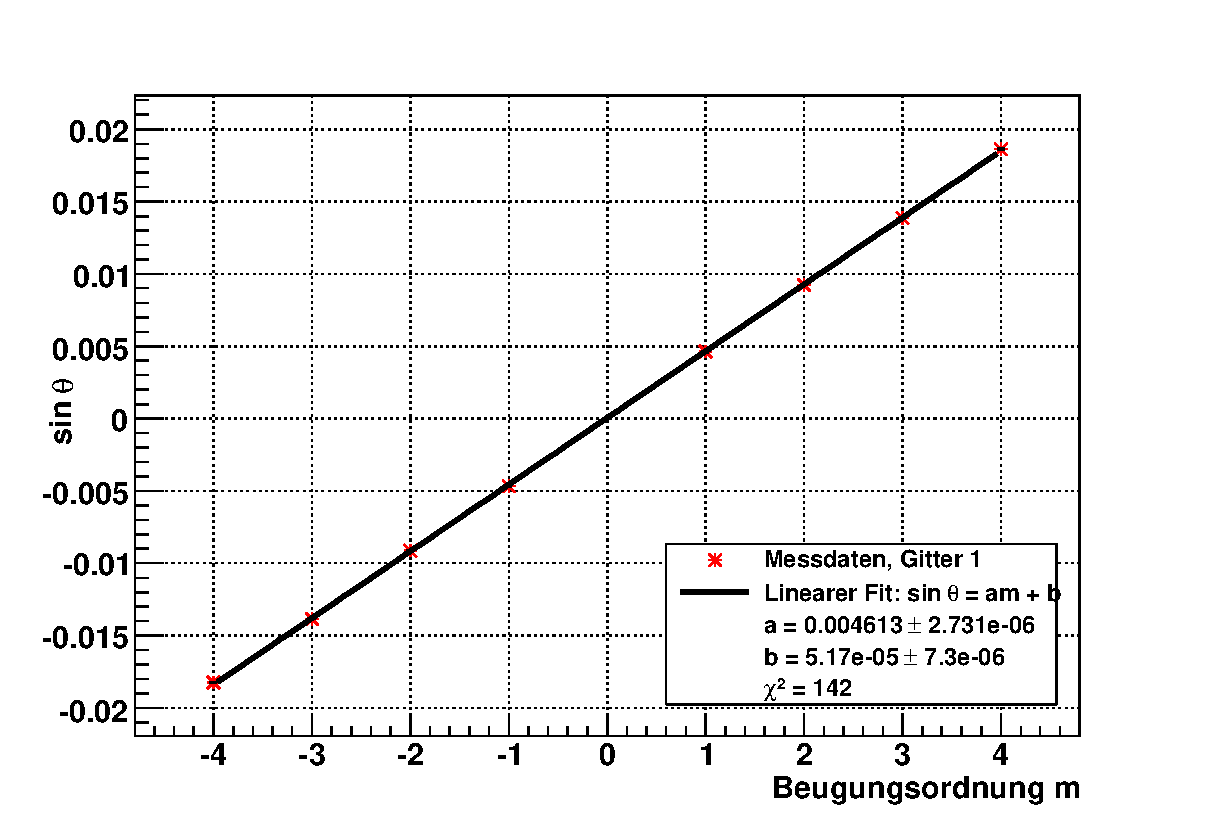
\includegraphics[width=0.7\linewidth]{pictures/gitter1.eps}
\caption{linerare Regresion der Daten zu Gitter 1}
\end{figure}

\begin{figure}[H]  
\centering
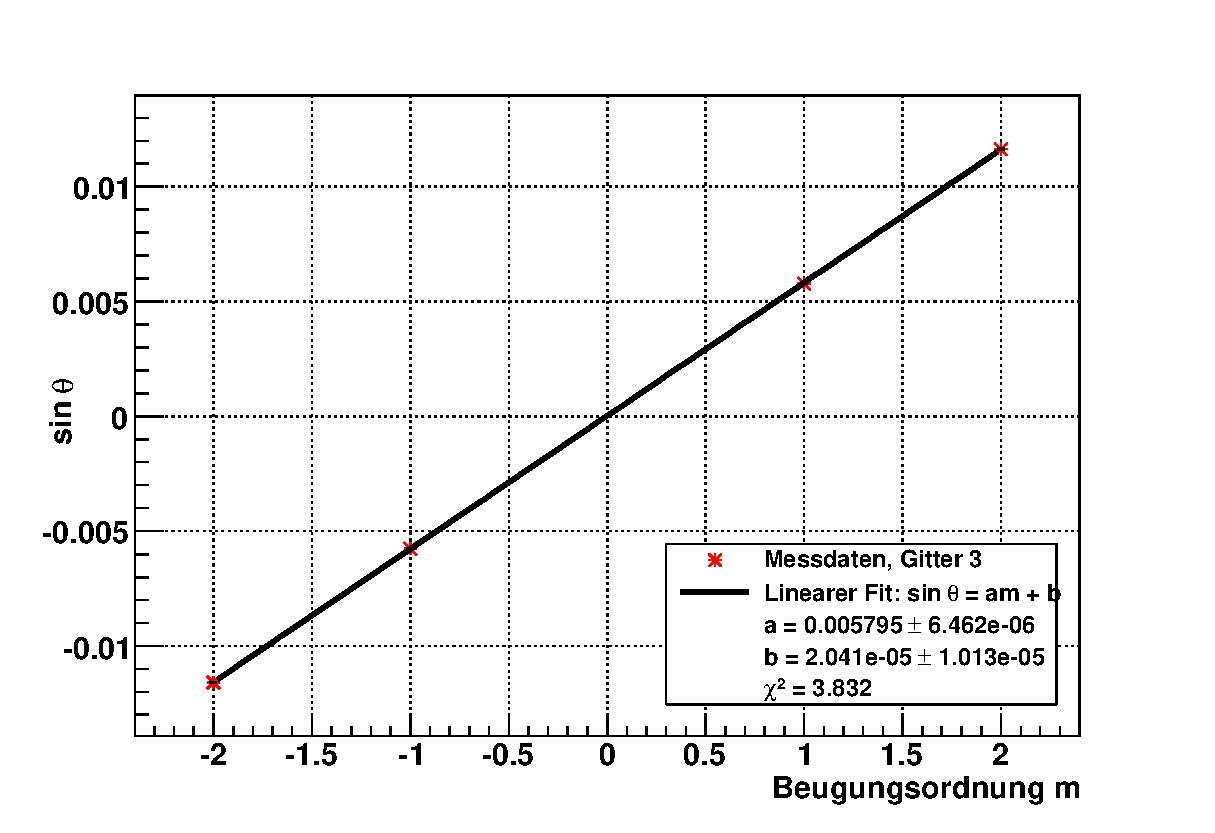
\includegraphics[width=0.7\linewidth]{pictures/gitter3.eps}
\caption{linerare Regresion der Daten zu Gitter 3}
\end{figure}

\begin{figure}[H]  
\centering
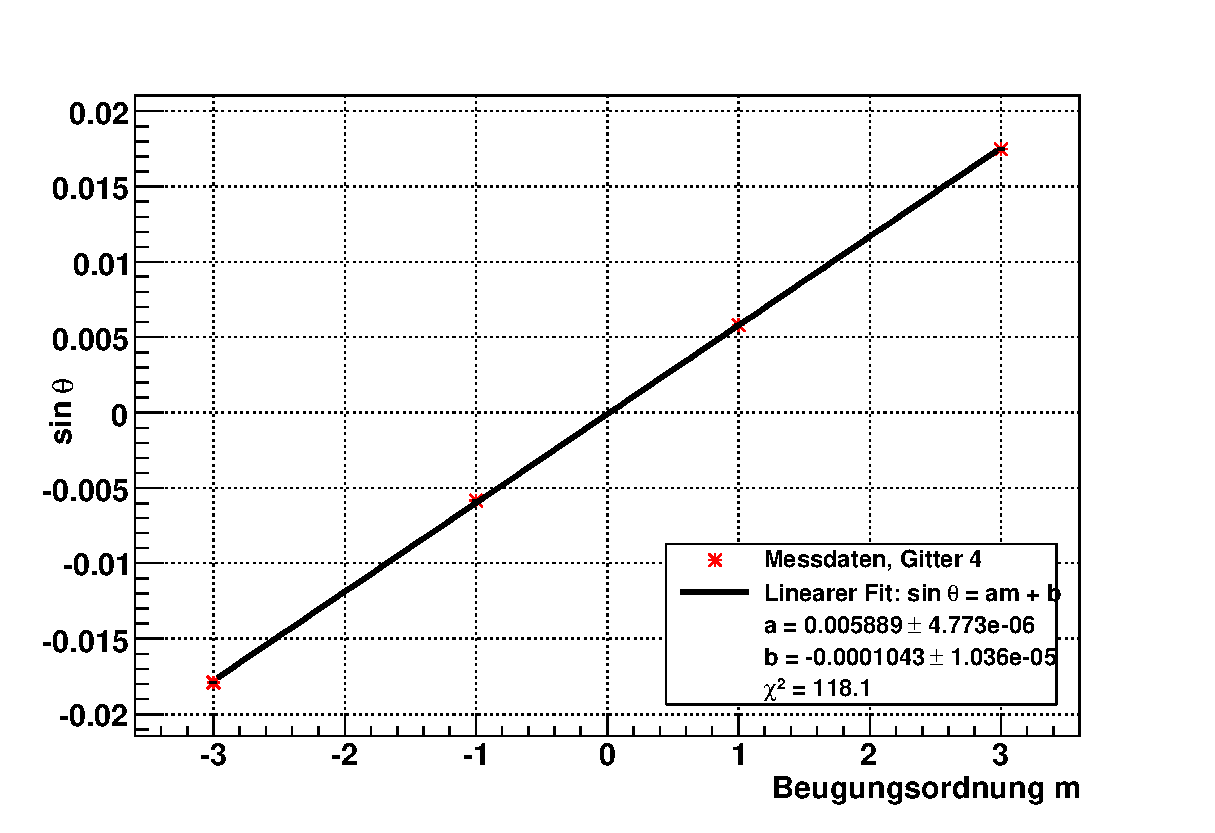
\includegraphics[width=0.7\linewidth]{pictures/gitter4.eps}
\caption{linerare Regresion der Daten zu Gitter 4}
\end{figure}

\begin{figure}[H]  
\centering
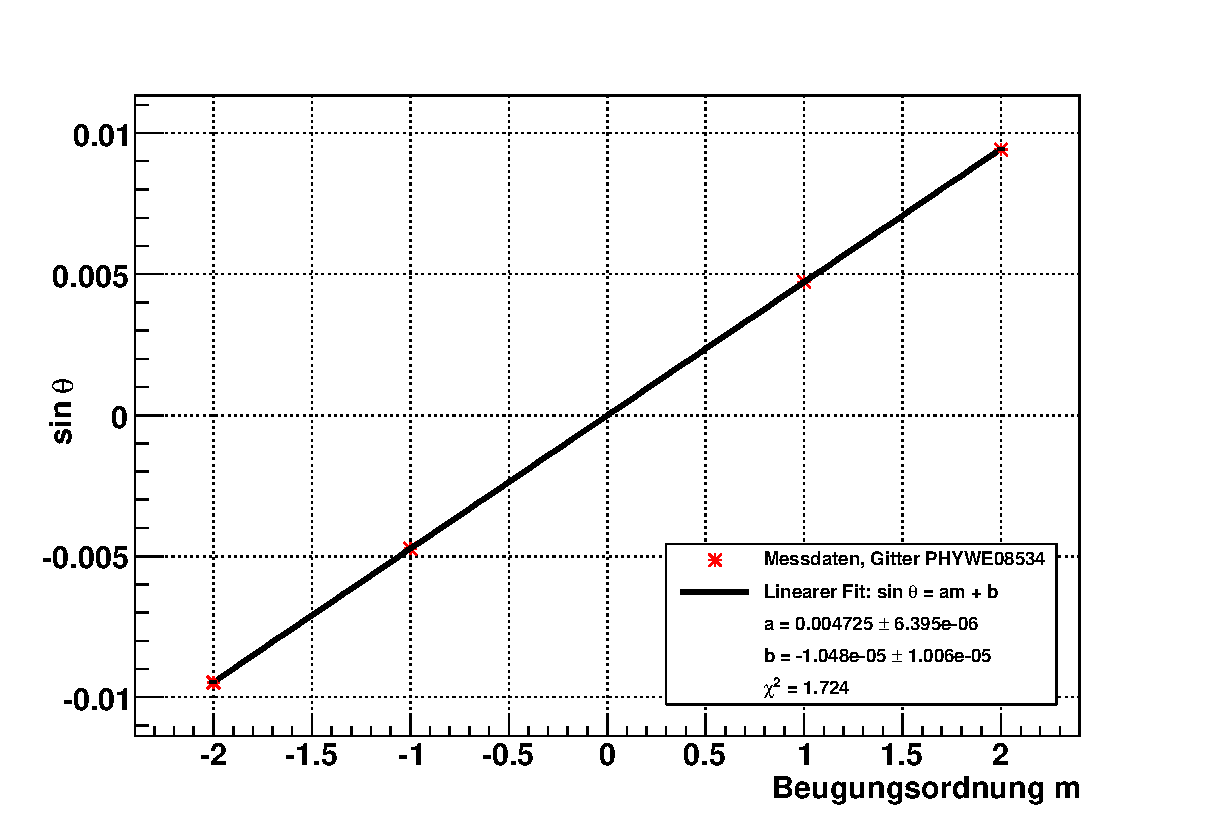
\includegraphics[width=0.7\linewidth]{pictures/phywe08534.eps}
\caption{linerare Regresion der Daten zu Gitter PHYWE08534}
\end{figure}

\begin{figure}[H]  
\centering
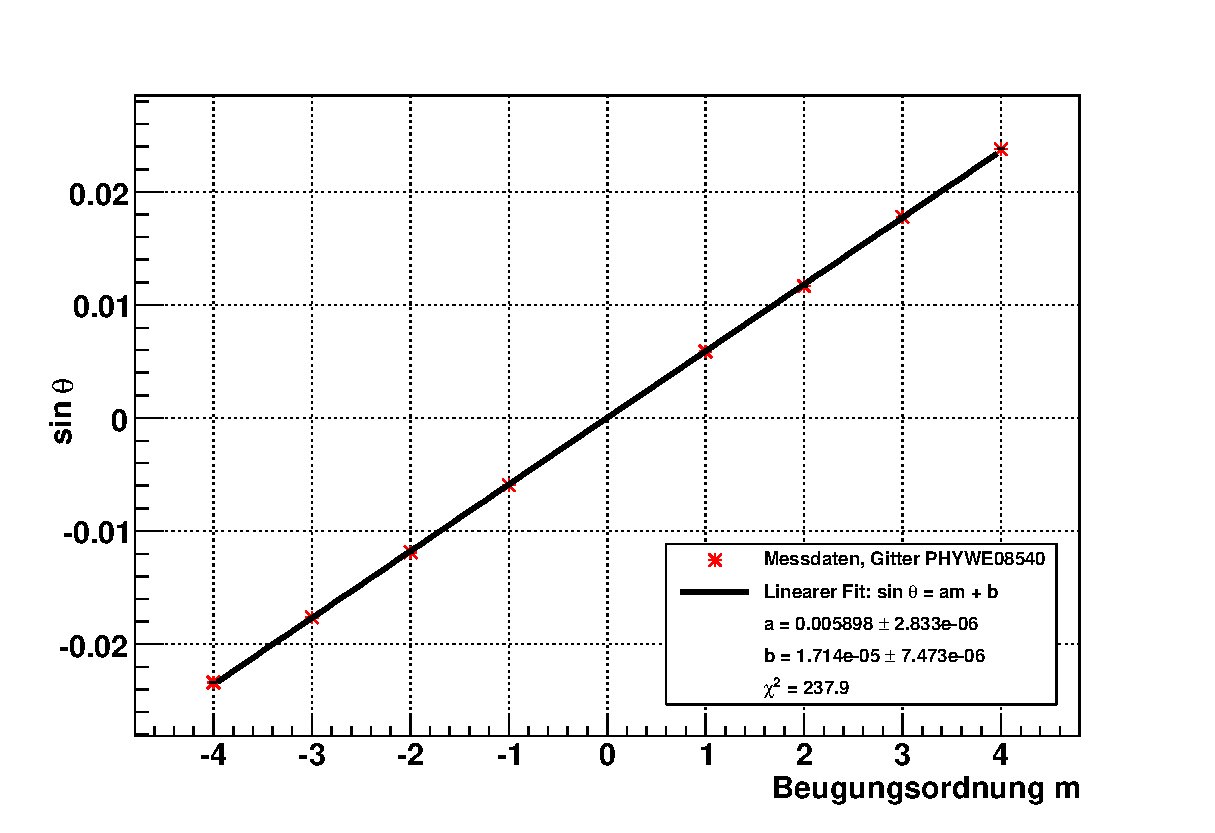
\includegraphics[width=0.7\linewidth]{pictures/phywe08540.eps}
\caption{linerare Regresion der Daten zu Gitter PHYWE08540}
\end{figure}

\subsection{Aperturfunktion und Verhältnis Spaltbreite zu -abstand von Gitter 1}

Wie in der Vorbereitung beschrieben nutzen wir zur Aproximation der Aperturfunktion $g$ die Fourierreihe:
\begin{align}
 g(x) = \sum_{j=0}^{m}{\sqrt{i_j}cos \left( \frac{x}{K} 2 \pi j \right)}
\end{align}

Die Intensitäten massen wir für jede Ordnung der Beugungsmaxima auf beiden Seiten und verwendeten den Mittelwert. Dabei schätzten wir einen Ablesefehler von $5mV$. 
\begin{align}
 \notag
I_0 &= (6585 \pm 5) mV \\
 \notag
I_1 &= (226 \pm 5) mV \\
 \notag
I_2 &= (178 \pm 5) mV \\
 \notag
I_3 &= (118 \pm 5) mV \\
 \notag
I_4 &= (58 \pm 5) mV
\end{align}

\begin{figure}[H]  
\centering
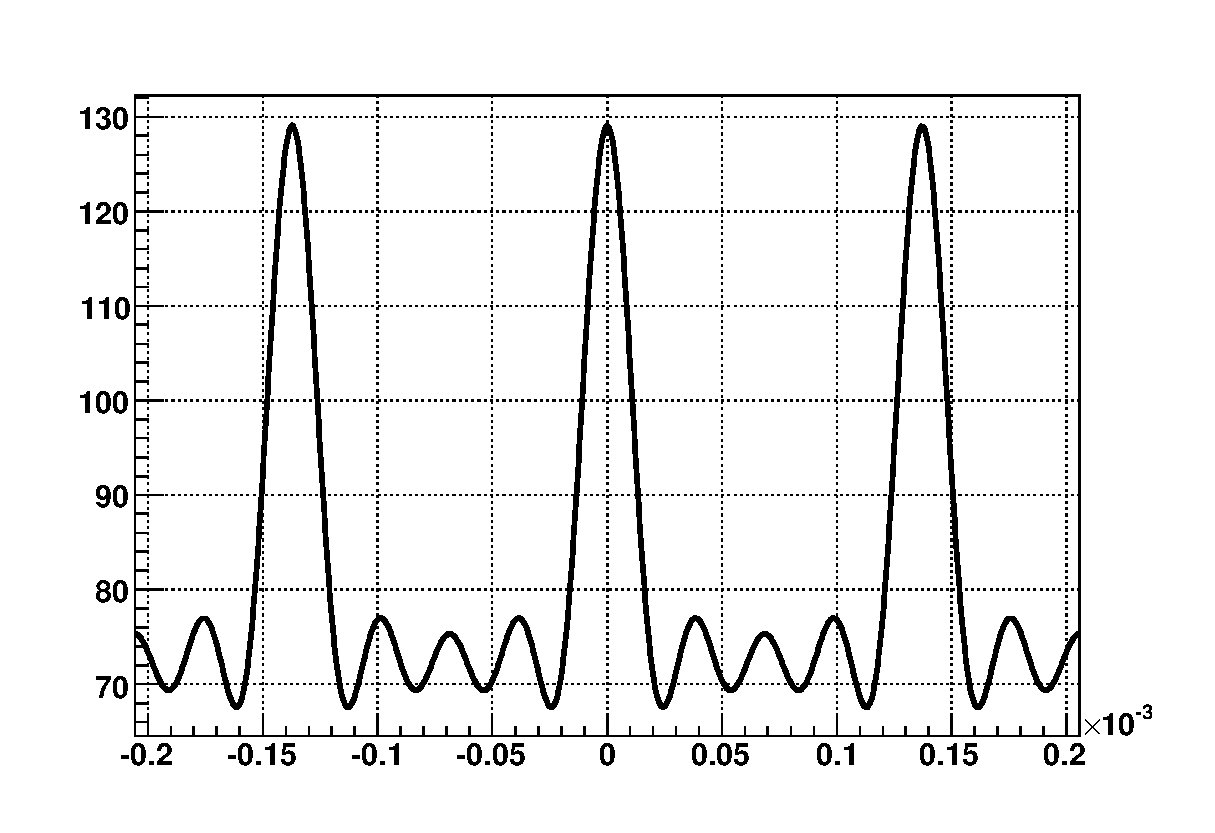
\includegraphics[width=0.7\linewidth]{pictures/apertur.eps}
\caption{Aproximation der Aperturfunktion für Gitter 1}
\end{figure}

Für das Verhältnis von Spaltbreite zu Spaltabstand benutzten wir den Wert der vollen Breite des halben Maximums (FWHM) als Wert für die Spaltbreite $w$. Der Spaltabstand $d$ berechnete sich dann mit Hilfe der Gitterkonstante $K$ aus $d= K - w$. Damit folgt direkt das Verhältnis $v=\frac{w}{d}$, mit dem Fehler $s_v=v\frac{s_d}{d}$:
\begin{align}
 \notag
v=0.19837 \pm 0,00019
\end{align}

\subsection{Auflösungsvermögen der Gitter}
Für den Durchmesser massen wir einen Wert von $d=(3 \pm 0,5)mm$. Die Anzahl der ausgeleuchteten Gitterlinien beträgt
$N=\frac{K}{d}$. Das Auflösungsvermögen folgt dann nach Gleichung \ref{auflösevermögen} 
\begin{align}
 a=Nm=\frac{K}{d}m
\end{align}

mit dem Fehler 
\begin{align}
 s_a=a\frac{s_N}{N}=a\sqrt{\left( \frac{s_d}{d}^2 \right) + \left( \frac{s_K}{K}^2 \right) }
\end{align}

Wir erhielten als Auflösungsvermögen:

\begin{align}
 \notag
a_1 &=  109 \pm  18\\
 \notag
a_3 &=  55,0 \pm  9,2\\
 \notag
a_4 &=  27,9 \pm  4,7\\
 \notag
a_{PHYWE08534} &= 90 \pm 15\\
 \notag
a_{PHYWE08540} &= 84 \pm 14
\end{align}

\subsection{Vergleich der Messung am Ultraschallphasengitter mit der Raman-Nath-Theorie}
Bei der Messung hatten wir leider einen nicht wegzubekommenden Peak neben dem Maximum der 0. Ordnung. Dieser wurde vermutlich von einer Reflexion
verursacht. Aus diesem Grund verwendeten wir nur die Positionsdaten der Maxima links von der 0. Ordnung.

Gemessen wurde der Spannungsabhängige Verlauf der einzelnen Beugungsordnungen. Um einen Vergleich mit der Raman-Nath-Theorie anstellen zu können müssen
die gemessenen Intensitätswerte auf $I_0(0) = J_0(0) = 1$ normiert werden. Um den Umrechnungsfaktor $b$ der die Generatorspannung in das passende Argument
der Besselfunktion zu erhalten nimmt man normalerweise den Spannungswert des erstem Minimums der 0. Ordnung und teilt ihn durch den $x$-Wert des ersten
Minimums der Besselfunktion selbiger Ordnung. Entsprechend verfährt man mit dem erstem Maximum der 1.Ordnung. 

Da sich in unserer Messung das erste Minimum der 0. Ordnung nicht bestimmen ließ basiert unsere Umrechnung nur auf den Daten der 1. Ordnung.
Als Umrechnungsfakor haben wir $b = 0,36824$ erhalten. Somit konnten wir die Quadrierten Besselfunktionen in die Graphen der einzelnen Ordnungen mit 
einfügen.

Für den Fehler auf die normierten Intensitäten erhält man:
\begin{align}
 s_{I/I_0} = \lvert I/I_0 \rvert ~ \sqrt{\left(\frac{s_I}{I}\right)^2 + \left(\frac{s_{I_0}}{I_0}\right)^2}
\end{align}

Für den Ablesefehler der Generatorspannung haben wir $0,1V$ angenommen.

Die Besselfunktionen wurden mittels der $J_n$ Implementierung aus dem Pythonpaket SciPy berechnet.

\begin{figure}[H]  
\centering
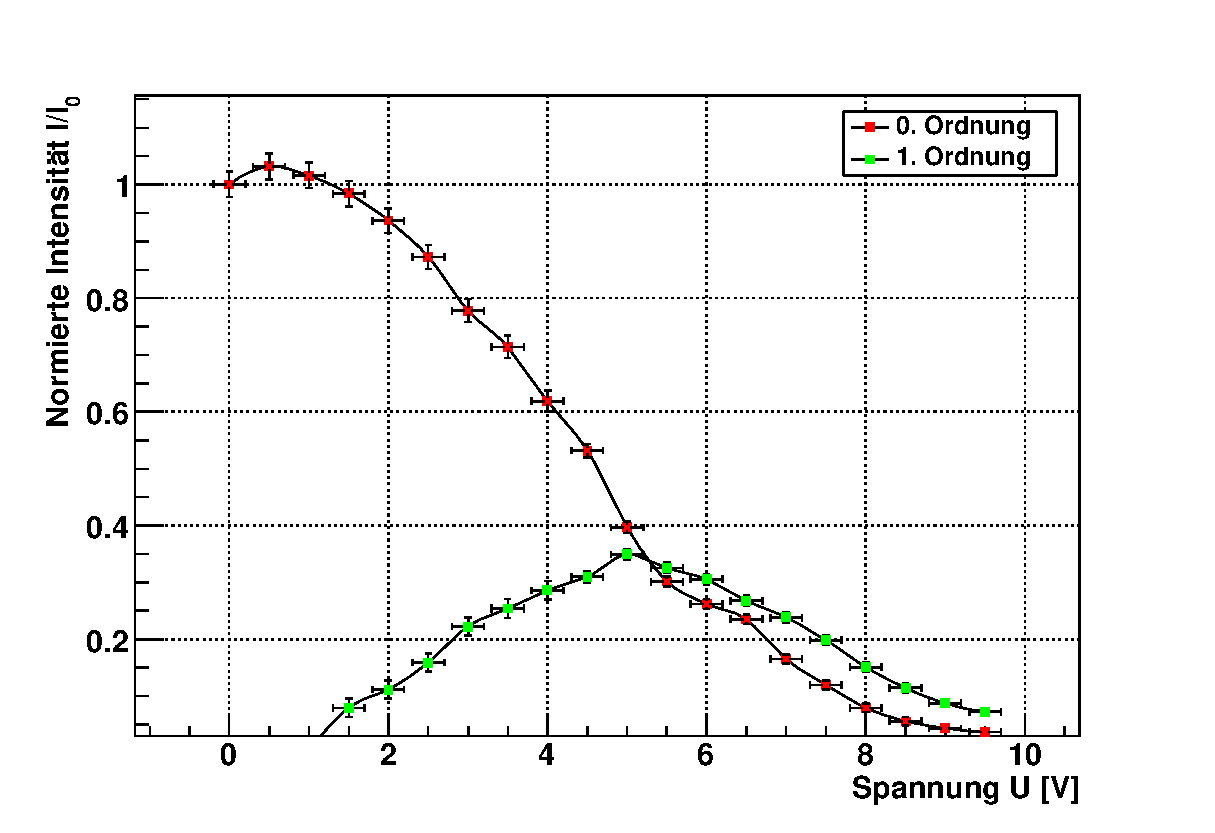
\includegraphics[width=0.9\linewidth]{pictures/raman0+1o.eps}
\caption{Verlauf der 0. und 1.Ordnung mit der Generatorspannung}
\end{figure}

\begin{figure}[H]  
\centering
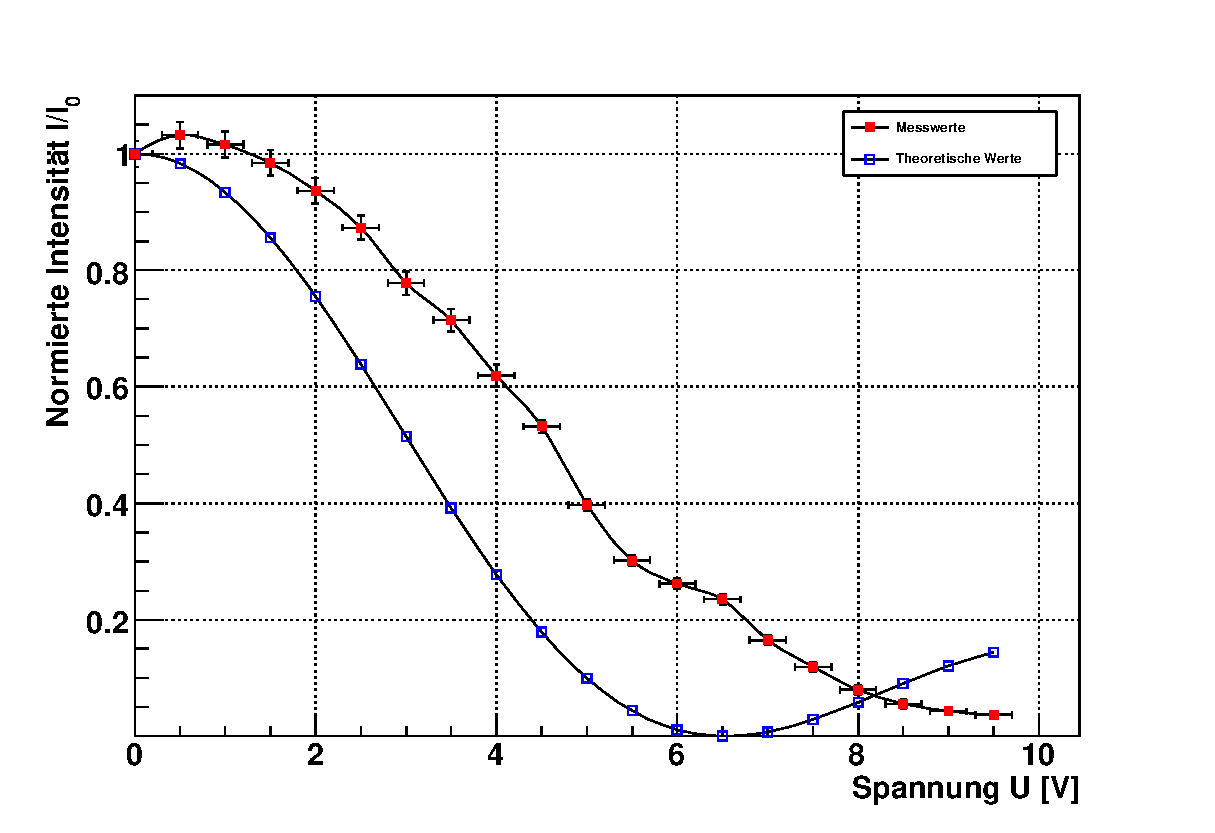
\includegraphics[width=0.9\linewidth]{pictures/raman0o.eps}
\caption{0.Ordnung und Besselfunktion $J^2_0$}
\end{figure}

\begin{figure}[H]  
\centering
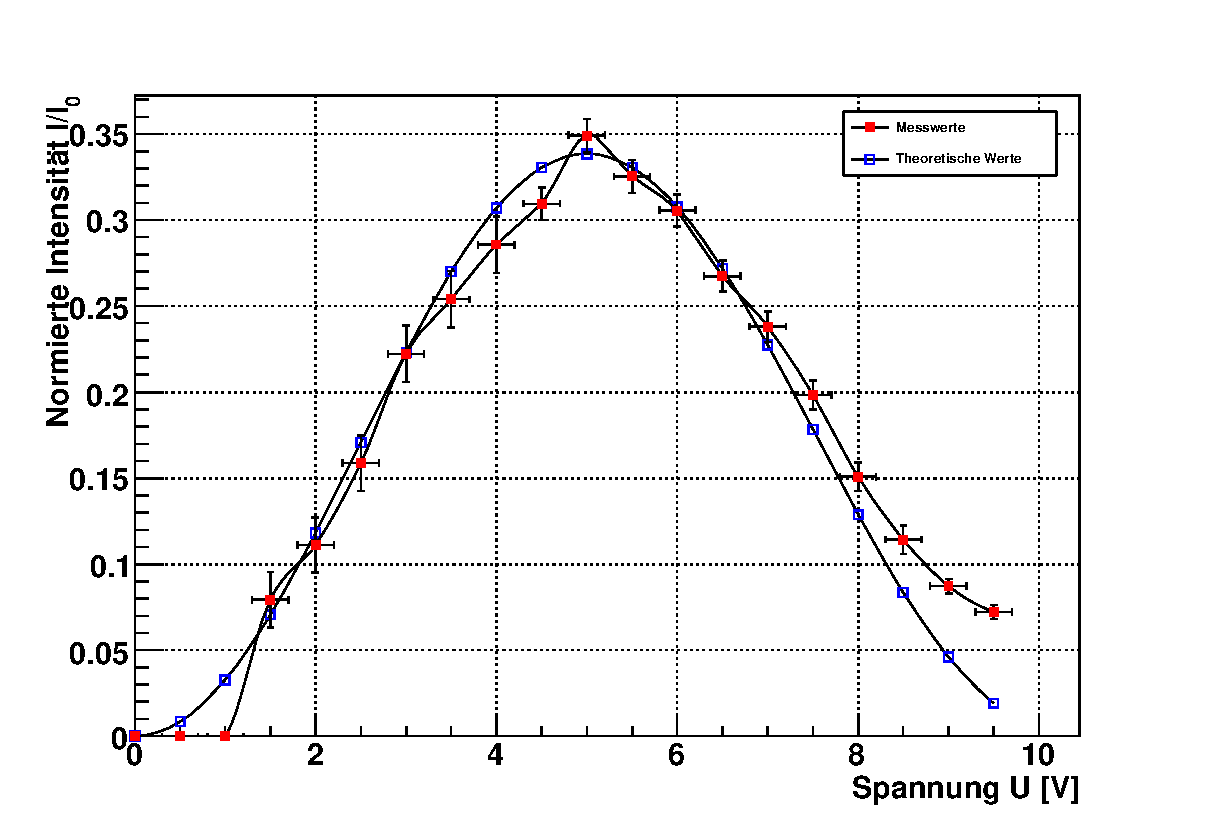
\includegraphics[width=0.9\linewidth]{pictures/raman1o.eps}
\caption{1.Ordnung und Besselfunktion $J^2_1$}
\end{figure}

\begin{figure}[H]  
\centering
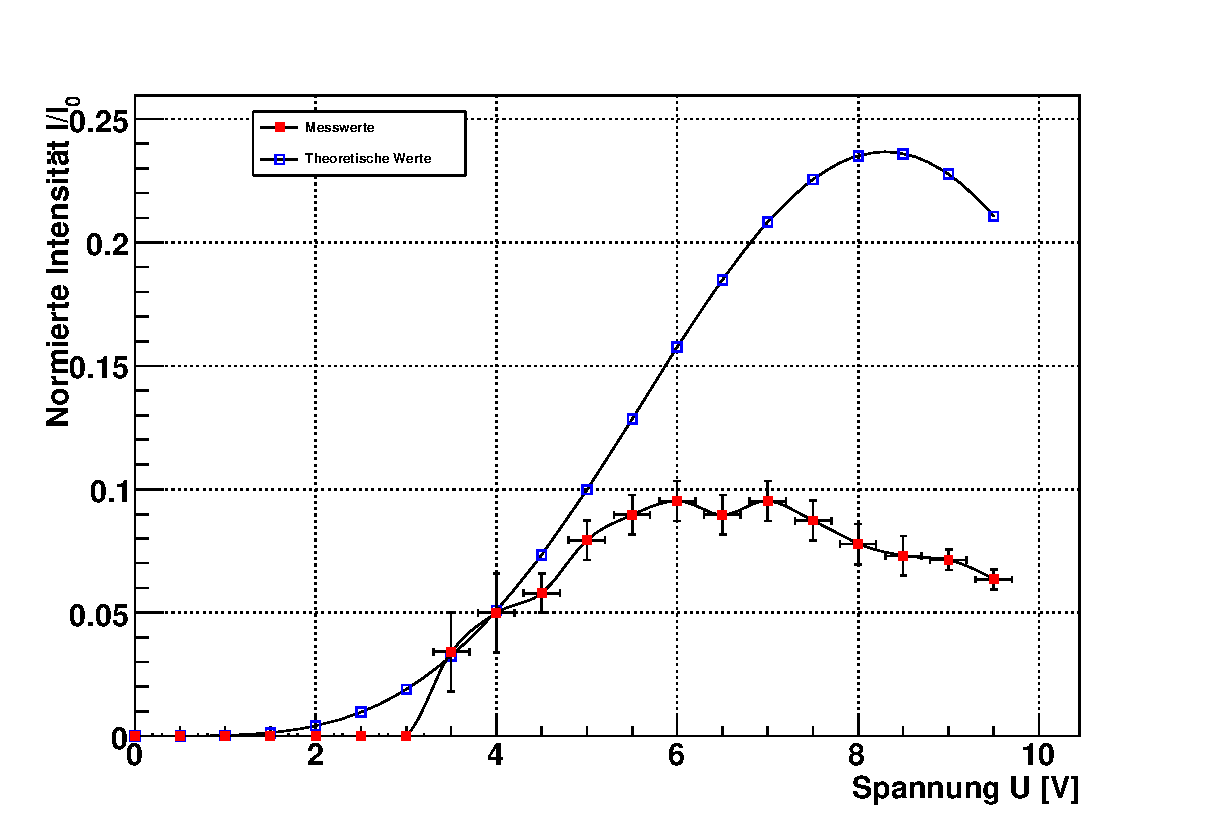
\includegraphics[width=0.9\linewidth]{pictures/raman2o.eps}
\caption{2.Ordnung und Besselfunktion $J^2_2$}
\end{figure}

\begin{figure}[H]  
\centering
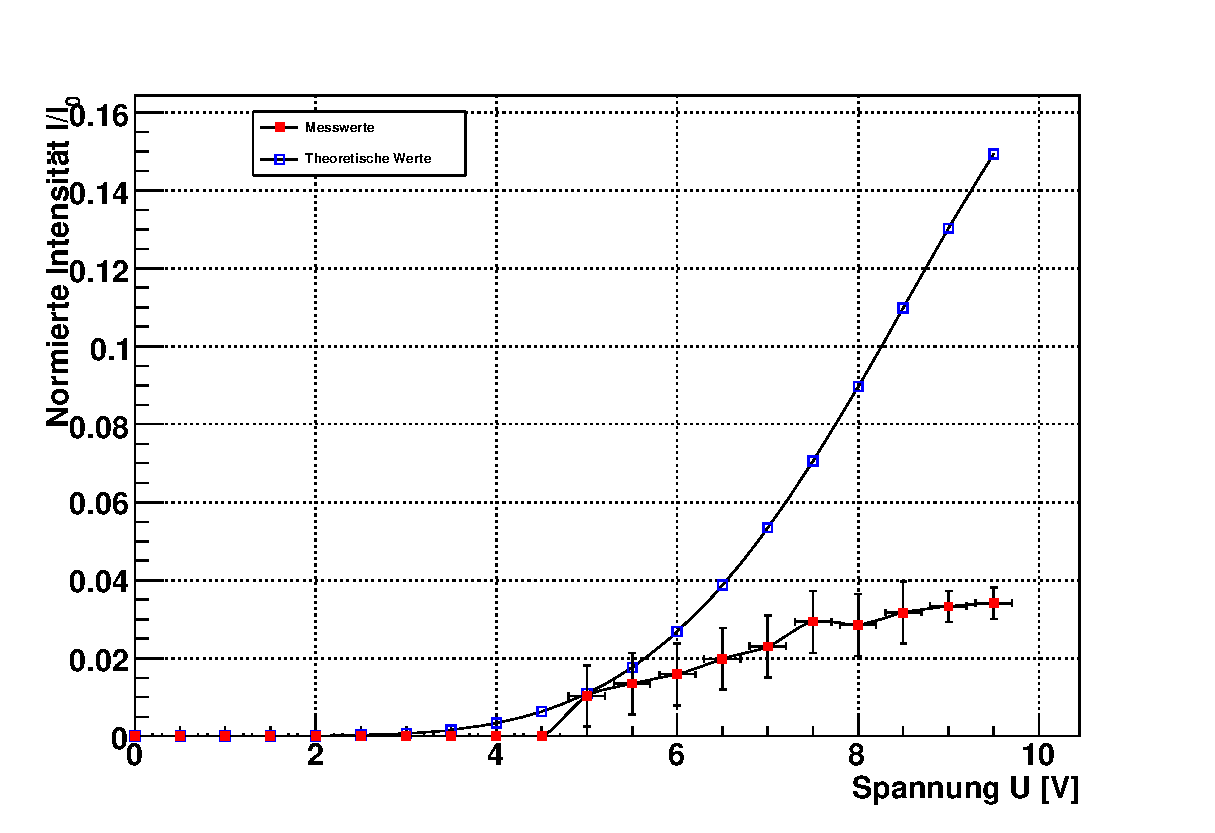
\includegraphics[width=0.9\linewidth]{pictures/raman3o.eps}
\caption{3.Ordnung und Besselfunktion $J^2_3$}
\end{figure}

\begin{figure}[H]  
\centering
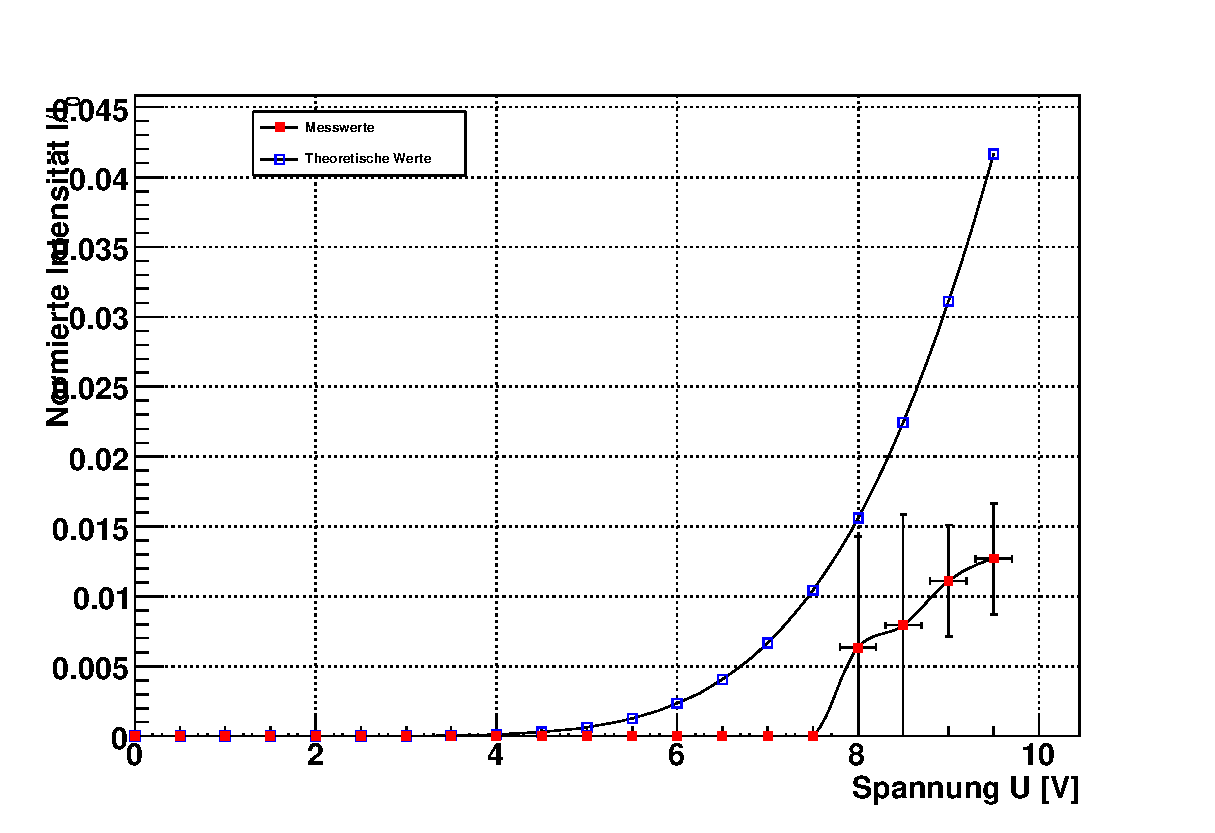
\includegraphics[width=0.9\linewidth]{pictures/raman4o.eps}
\caption{4.Ordnung und Besselfunktion $J^2_4$}
\end{figure}


\subsection{Bestimmung der Schallwellenlänge}
Durch die Veränderung des Versuchsaufbaus (Einsetzen der Ultraschallzelle) musste die Eichung der Zeitachse aufs neue durchgeführt werden.
Hierzu setzten wir das Gitter $R$ (80 Striche/cm) hinter die Ultraschallzelle in der Strahlengang und bestimmten wieder
die Zeitunterschiede zw. 0. und $m$-ter Ordnung.

\begin{figure}[H]  
\centering
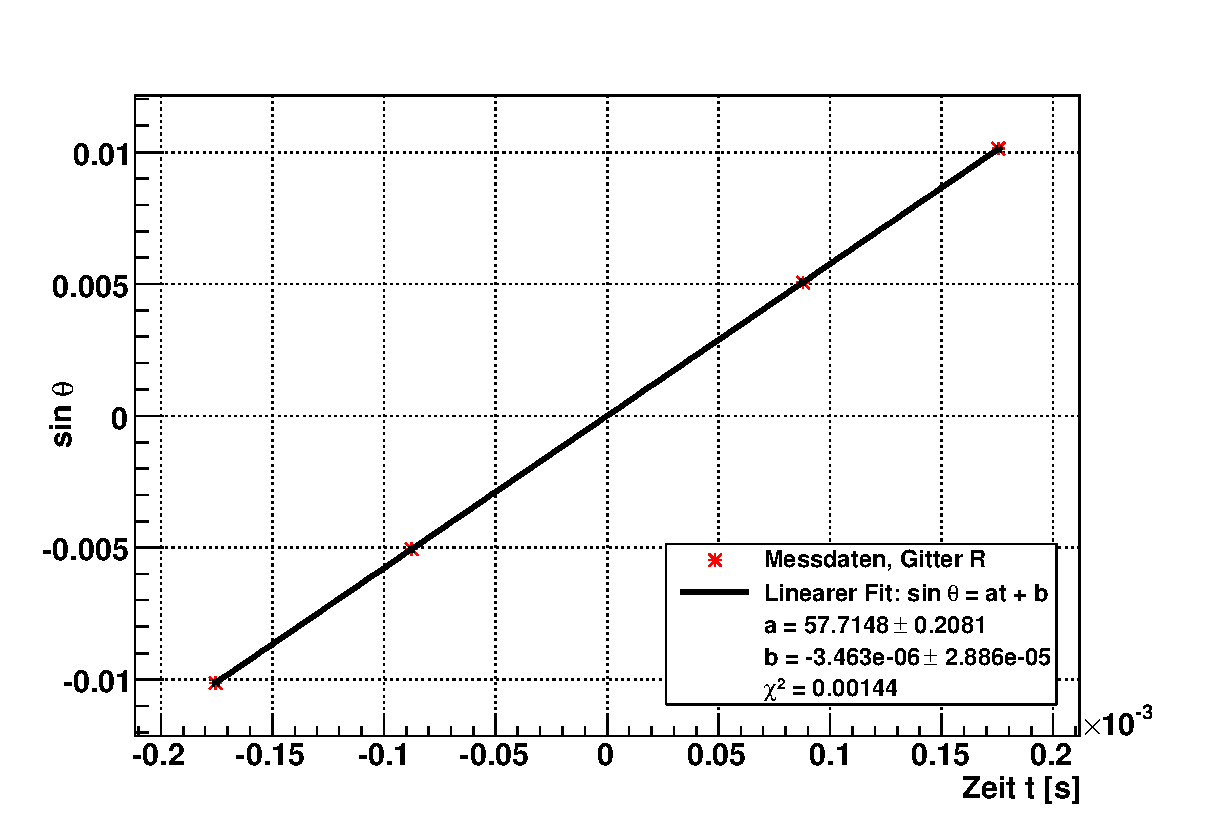
\includegraphics[width=0.9\linewidth]{pictures/schall_r.eps}
\caption{Eichung der Zeitachse mit Gitter R}
\end{figure}

Durch lineare Regression erhält man den Zusammenhang zw. Zeit und $\sin\theta$ : $\sin\theta = a~t + b$ mit $a = (57,7 \pm 0,2) \frac{1}{s}$
und $b = (0,4 \pm 2,9)\times 10^{-5}$.

Die Schallwellenlänge lässt sich dann analog zur Gitterkonstante mit linearer Regression aus dem Graph $\sin\theta$ gegen $m$ berechnen:
\begin{align}
 \Lambda = \frac{\lambda}{a} = (5.678 \pm 0,052)*10^{-4} m
\end{align}

Mit der Schallgeschwindigkeit in Isooktan von $c = 1111 \frac{m}{s}$ lässt sich die Ultraschallfrequenz berechnen zu:
\begin{align}
 f = \frac{c}{\Lambda} = (1.957 \pm 0.018) MHz
\end{align}

\begin{figure}[H]  
\centering
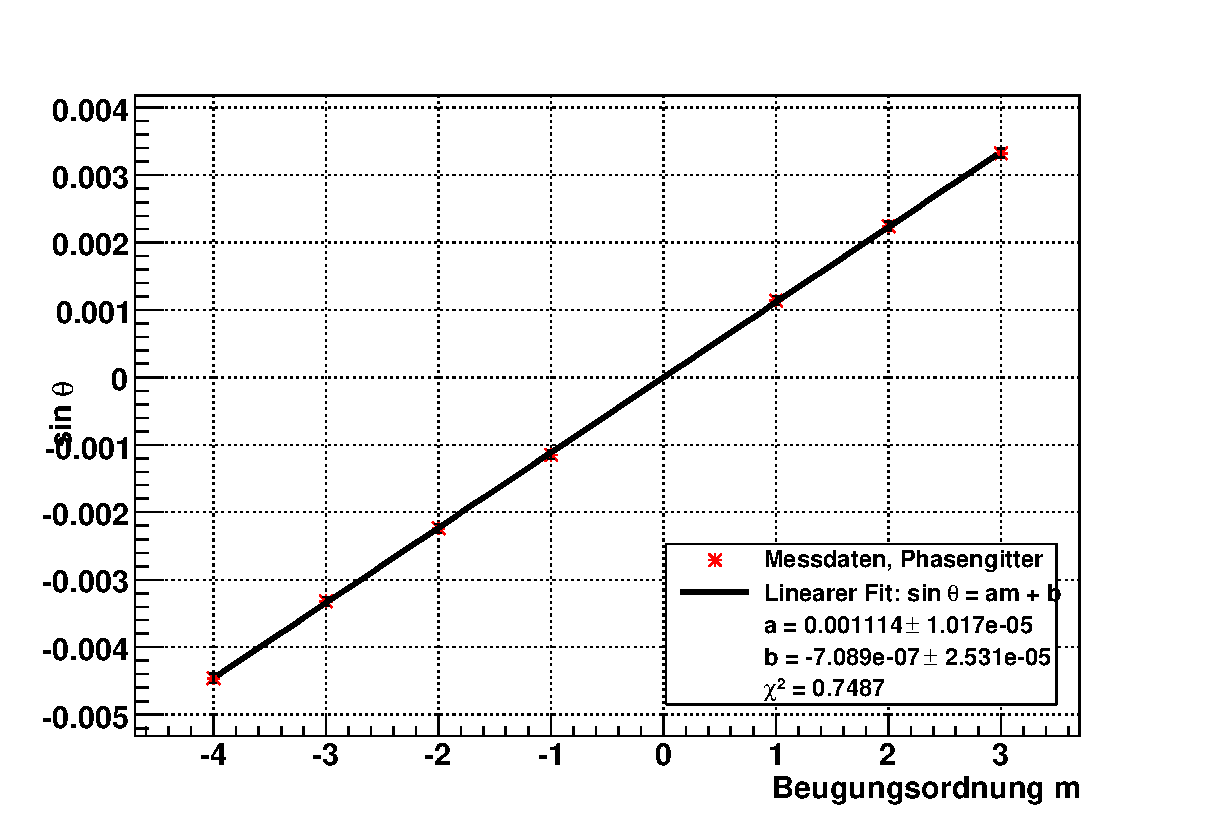
\includegraphics[width=0.9\linewidth]{pictures/phasengitter.eps}
\caption{Ultraschallphasengitter}
\end{figure}

\section{Zusammenfassung}

\end{document}
